\documentclass[aps,prd,10pt,onecolumn,nofootinbib,superscriptaddress,floatfix]{revtex4-2}

\usepackage[T1]{fontenc}
\usepackage{lmodern}
\usepackage[utf8]{inputenc}
\input{glyphtounicode}
\pdfgentounicode=1
\usepackage{amsmath,amssymb,amsthm,mathtools}
\usepackage{bm}
\usepackage{graphicx}
\usepackage{placeins}
\usepackage[hidelinks]{hyperref}

\newtheorem{theorem}{Theorem}
\newtheorem{corollary}{Corollary}

\begin{document}
\raggedbottom

\title{Can a Wormhole Induce a Monopole?}

\author{Sergei Slobodov}
\email{sergei@slobodov.com}
\noaffiliation

\date{\today}

\begin{abstract}
Dai and Stojkovic proposed that a body orbiting near one mouth of a traversable
wormhole could make the mass seen near the other mouth rise and fall.  We show
that their static solutions do not establish this signal.  In
electromagnetism, Stokes' theorem fixes the charge measured on an observer-side
surface unless current crosses that surface.  On the stationary background
used in the proposal, the corresponding first-order gravitational quantity is
the mass perturbation and obeys the same source balance.  It therefore cannot
track the source's orbital radius unless first-order energy crosses the
measuring surface.  Higher multipoles, waves, and dynamical throat effects
remain possible.
\end{abstract}

\maketitle

% ============================================================
\section{Introduction}
\label{sec:introduction}
% ============================================================

A field sourced near one mouth of a traversable wormhole can influence fields
near the other.  The narrower question here is whether moving that source can
change the mass an observer measures near the opposite mouth, when neither
matter nor the fields supporting the wormhole carry first-order energy across
the measuring surface.  We answer it for the mass monopole, to first order in
the source mass $\mu$.

Dai and Stojkovic (DS) proposed such a modulation in a short-throat geometry
made from two Schwarzschild exteriors.  A static matching calculation assigns
the observer side a mass-like coefficient proportional to the inverse source
radius.  DS then replace that radius by the radius of an eccentric orbit and
interpret the resulting periodic $1/r^2$ acceleration as a wormhole signature
near Sgr~A* \cite{DaiStojkovic2019Observing}.  Krasnikov objected that the
spherical monopole region is Schwarzschild by Birkhoff's theorem
\cite{Krasnikov2020CommentObserving}.  DS replied that an eccentric orbit is
nonspherical and may be viewed as a sequence of monopoles
\cite{DaiStojkovic2020ReplyObserving}.  The same acceleration law was later
used in sensitivity estimates \cite{SimonettiEtAl2021SensitiveSearches}.

The $\ell=0$ part of the perturbation in a connected vacuum region is a
constant mass variation plus gauge, and its normalized surface charge obeys a
local balance law, which in turn fixes what a genuine signal would require.
The relevant distinction is between a family of static solutions and
successive states of one on-shell dynamical history.

We first state that distinction in Maxwell theory, where it follows
immediately from Stokes' theorem: each mouth carries a flux of its own,
changed only by current crossing its own surface.  We then use the Iyer--Wald
linearized time-translation charge for
gravity \cite{IyerWald1994NoetherCharge}.  The argument is local to the chosen
measuring worldtube, and applies equally when that surface bounds no compact
interior and when the wormhole has a single asymptotic end.

We use geometrized units $G=c=1$, denote the background mass by $M$ and write
$r_g=2M$, and work to first order in the small mass ratio
\begin{equation}
  \epsilon=\frac{\mu}{M}\ll1.
\end{equation}

% ============================================================
\section{The DS static family and its dynamical use}
\label{sec:ds-model}
% ============================================================

DS join two copies of the Schwarzschild exterior,
\begin{equation}
  d\bar s^2=-f(r)dt^2+f(r)^{-1}dr^2+r^2d\Omega^2,
  \qquad f(r)=1-\frac{r_g}{r},
  \label{eq:background}
\end{equation}
at spheres $r=R>r_g$.  A small source of mass $\mu$ is placed at radius
$r_1=A>R$ in the ``other'' exterior, and $r_2$ denotes the observer-side
radius.  Later arXiv revisions \cite{DaiStojkovic2019ObservingV2,
DaiStojkovic2019ObservingV3} give the observer-side monopole
\begin{equation}
  h^{\mathrm{our}}_{tt}=\frac{2b}{r_2},
  \qquad
  h^{\mathrm{our}}_{rr}=\frac{2b r_2}{(r_2-r_g)^2},
  \qquad
  b=\frac{\mu R}{A},
  \label{eq:ds-observer-mode}
\end{equation}
This is the strongest form of the proposal: the observer field is a vacuum mass
perturbation, while the predicted acceleration is unchanged.  We use it
throughout.  DS identify $b$ as an effective mass at the observer mouth.%
\footnote{The journal field instead uses
$b_{tt}=\mu R/A$ and
$b_{rr}=\mu A(R-r_g)^2/[R(A-r_g)^2]$
\cite{DaiStojkovic2019Observing}.  For $A>R$,
$\delta G^{r}{}_{r}=2(b_{tt}-b_{rr})/[f(r_2)r_2^3]\ne0$, so this field is off
shell; later revisions set $b_{rr}=b_{tt}$.  Their displayed source-side
annulus $R<r<A$, with $h_{tt}=2\mu/A$ and $h_{rr}=0$, is also off shell,
$\delta G^{r}{}_{r}=2\mu r_g/[Af(r)r^3]\ne0$.  Krasnikov likewise notes that
the source DS cite says the perturbation vanishes inside the orbit
\cite{Krasnikov2020CommentObserving}.  We therefore grant the strongest
on-shell completion, with $b$ the $\ell=0$ mass coefficient.}

Far from the mouth, the associated acceleration is
\begin{equation}
  a_{\mathrm{DS}}\simeq-\frac{b}{r_2^2}
  =-\frac{\mu R}{A r_2^2}.
  \label{eq:ds-acceleration}
\end{equation}
For an eccentric orbit with periapsis $r_p$ and apoapsis $r_a$, the proposed
acceleration amplitude is therefore
\begin{equation}
  |\Delta a_{\mathrm{DS}}|
  =\mu R\left(\frac{1}{r_p}-\frac{1}{r_a}\right)\frac{1}{r_2^2}.
  \label{eq:ds-delta-a}
\end{equation}
This step replaces $A$ in a static boundary-value solution by $A(t)$.  It is
valid only if the different static solutions belong to one dynamically
reachable charge sector.

Substituting $b\to b(t)$ directly into Eq.~\eqref{eq:ds-observer-mode} already
exposes the difficulty.  The time--radial component of the linearized Einstein
tensor is then
\begin{equation}
  \delta G^{r}{}_{t}=\frac{2\dot b}{r_2^{2}},
  \label{eq:momentum-constraint}
\end{equation}
which must vanish in vacuum, forcing $\dot b=0$.  When a source is present,
$\delta G^{r}{}_{t}=8\pi\,\delta T^{r}{}_{t}$ integrates over the sphere to
$\dot b=\oint\delta T^{r}{}_{t}\,dA$: the coefficient changes at exactly the
rate energy crosses the measuring sphere.  The rest of this paper reaches the
same conclusion for a perturbation of any angular dependence, and in a
manifestly gauge-invariant way, so
that the varying quantity is an observable rather than a coordinate
coefficient.  The next two sections do so.%
\footnote{The calculation assumes a timelike cut $R>r_g$ and a uniform
linearization.  Since the mode in Eq.~\eqref{eq:ds-observer-mode} is a mass
perturbation, smallness at the cut requires
$2\mu R/[A(R-r_g)]\ll1$.  Thus the choice $R=r_g$, discussed by DS, lies
outside this perturbative regime.}

% ============================================================
\section{Maxwell prototype: a worldtube balance}
\label{sec:maxwell}
% ============================================================

Let $F$ be the Maxwell field and $j$ the electric current.  For a closed
two-surface $S$, define
\begin{equation}
  Q[S]=\frac{1}{4\pi}\int_S\star F.
  \label{eq:maxwell-charge}
\end{equation}
Let $S_t$ be a smooth family of measuring surfaces and let
$\mathcal T=\bigcup_{t\in[t_1,t_2]}S_t$ be the timelike three-surface they
sweep out.

Frolov and Novikov proved the corresponding balance for a static wormhole,
concluding that the flux through the handle cannot change until charged
particles pass through it, and that motion of charges in the external space
leaves it unaltered \cite{FrolovNovikov1990PhysicalEffects}.  The surface that
matters for the DS claim is a different one---an observer-side sphere
enclosing a single mouth---so we restate the identity for an arbitrary
measuring family.

\begin{theorem}[Measuring-surface balance, after Frolov and Novikov]
\label{thm:maxwell}
If $\partial\mathcal T=S_{t_2}-S_{t_1}$, then
\begin{equation}
  Q[S_{t_2}]-Q[S_{t_1}]=\int_{\mathcal T}\star j.
  \label{eq:maxwell-balance}
\end{equation}
In particular, the measured flux is constant whenever no electric current
crosses $\mathcal T$.
\end{theorem}

\begin{proof}
Integrate $d\star F=4\pi\star j$ over $\mathcal T$ and apply Stokes' theorem.
Each $S_t$ is arbitrary, and may bound no compact region.
\end{proof}

Figure~\ref{fig:worldtube} makes explicit which surface is being followed:
$\mathcal T$ is the history of the observer's measuring surface, not a cut
through the throat.

\begin{figure}[!ht]
  \centering
  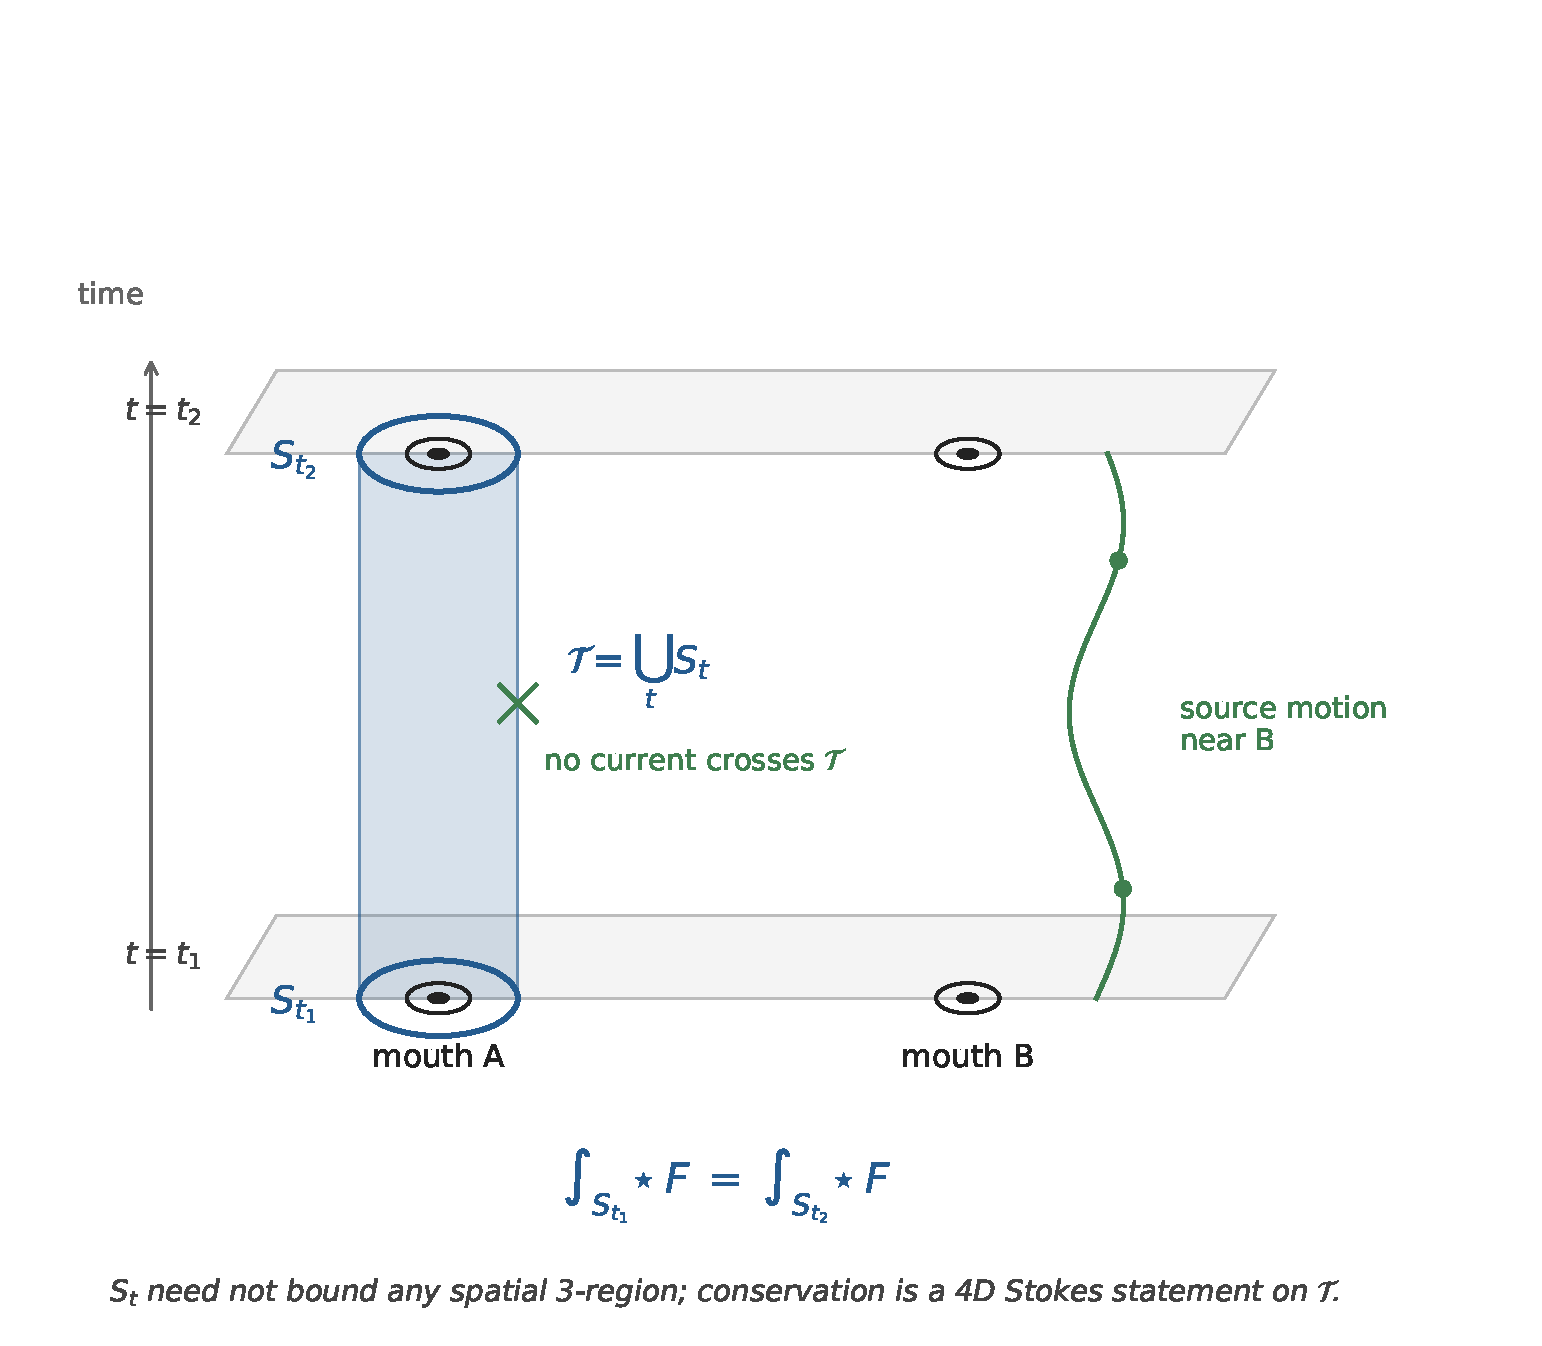
\includegraphics[width=0.72\textwidth,trim=0 35 0 55,clip]{fig_worldtube_stokes.pdf}
  \caption{A measuring surface $S_t$ is compared at $t_1$ and $t_2$ through
  its spacetime history $\mathcal T=\bigcup_tS_t$.  If no current crosses
  $\mathcal T$, Stokes' theorem gives equal Maxwell fluxes on the endpoint
  surfaces even when the source moves near the other mouth.  The gravitational
  argument uses the same geometry with the first-order Killing charge in place
  of the Maxwell flux.}
  \label{fig:worldtube}
\end{figure}

In a source-free region, $d\star F=0$ and the flux is a period of the closed
form $\star F$.  Wormhole topology permits a nonzero source-free period---the
classical ``charge without charge'' sector
\cite{MisnerWheeler1957ClassicalPhysics}.  Its value is initial or boundary
data preserved by source-free evolution.

The magnetic period is fixed more rigidly still.  Since $dF=0$ identically,
$\int_SF$ is unchanged by any evolution, including transit of charged matter
through the throat \cite{FrolovNovikov1990PhysicalEffects}.  A wormhole
threaded by magnetic flux accordingly presents a static monopole field at each
mouth, and searches in that sector treat the flux as fixed data
\cite{PiotrovichEtAl2024WormholeCandidates}.

Fixed monopole flux still permits a nonzero cross-mouth field.
Figure~\ref{fig:fixed-sector-field} illustrates this distinction in a flat
spherical thin-shell wormhole formed by identifying two copies of the exterior
of a ball in flat space at their boundary sphere
\cite{Visser1995LorentzianWormholes}.  A Legendre expansion with
the $\ell=0$ harmonic coefficient fixed still contains an angular response on
the opposite side.

The measuring surface must be specified.  A charge crossing a throat cut can
change the flux through that cut without changing the flux through a fixed
observer sphere if the charge remains between the throat and the sphere.  If
the charge later crosses the observer sphere, Eq.~\eqref{eq:maxwell-balance}
changes the measured flux by the ordinary current term.

In the DS electrostatic family a point charge $q$ sits at radius $A$ in the
other space, and the monopole flux through an observer-side sphere is, in the
normalization of Eq.~\eqref{eq:maxwell-charge},%
\footnote{DS use an unnormalized flux and a charge parameter differing by the
same factor of $4\pi$; the ratio $Q_2/q$ in Eq.~\eqref{eq:ds-electric} is
unchanged.}
\begin{equation}
  Q_2^{\mathrm{DS}}(A)=\frac{qR}{2A}.
  \label{eq:ds-electric}
\end{equation}
During motion confined near the other mouth, no current crosses the fixed
observer-side worldtube.  The theorem therefore holds $Q_2$ constant, whereas
Eq.~\eqref{eq:ds-electric} varies it with $A$.  The fixed-$A$ fields may be
valid static boundary-value solutions, but different values of $A$ select
different conserved-flux data.  They are not successive states of a single
Maxwell evolution.  This is the local worldtube form of the fixed
wormhole-charge prescription used in
Ref.~\cite{Krasnikov2008ElectrostaticInteraction}.

Theorem~\ref{thm:maxwell} applies to a sphere around either mouth, so each
carries a flux of its own, changed only by current crossing that sphere.

\begin{figure}[!ht]
  \centering
  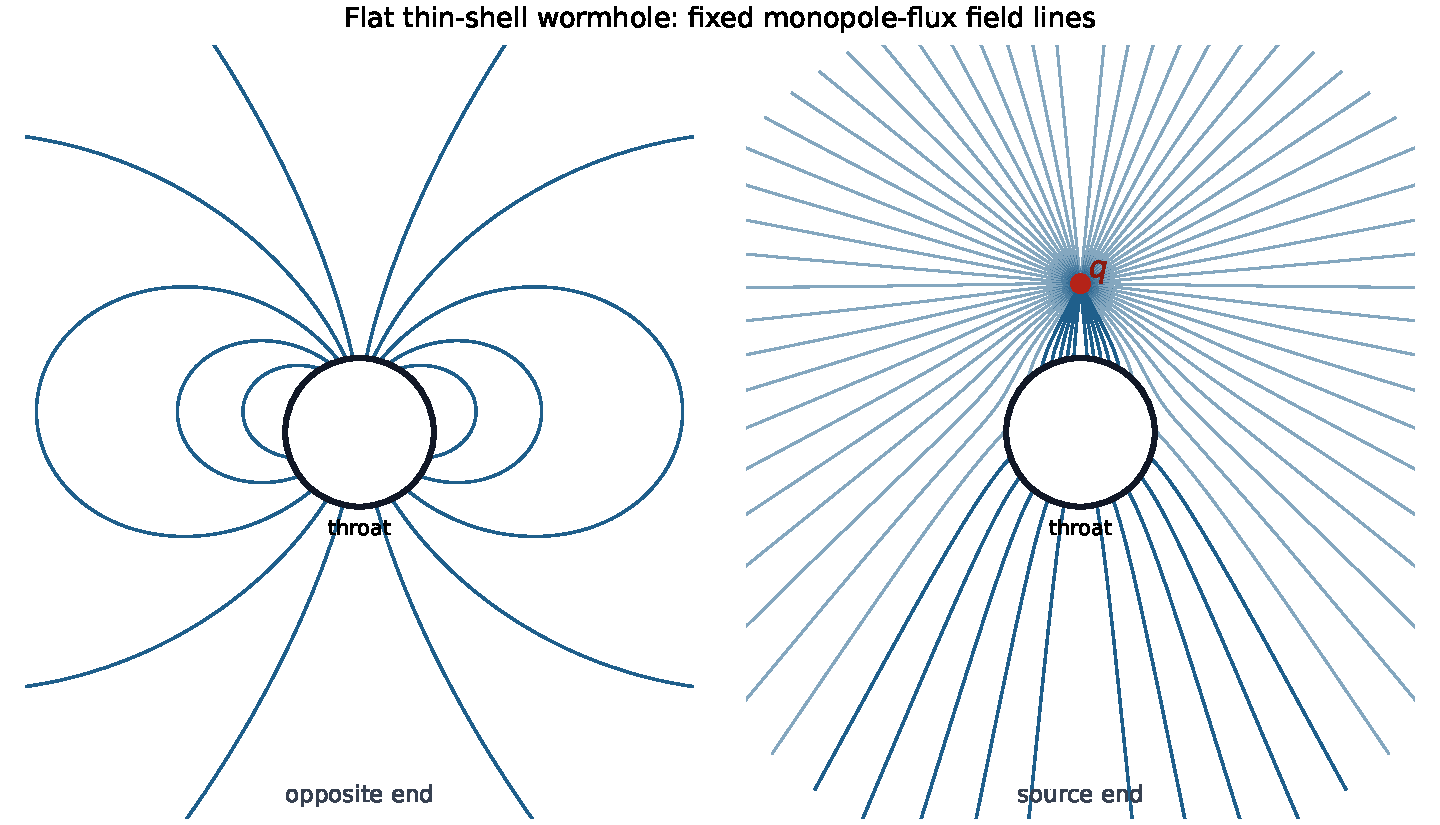
\includegraphics[width=0.88\textwidth]{fig_thinshell_fixed_monopole_flux_v7.pdf}
  \caption{Illustrative fixed-sector Maxwell field.  The two panels are the
  two exterior charts, and the black circles represent the same identified
  throat sphere.  A charge in the source chart produces a nonzero field in the
  opposite chart, but in the chosen zero-flux sector throat-crossing field
  lines return through another angular band.  The integrated flux and the
  opposite-side Coulomb monopole are fixed by the chosen sector; the balance
  theorem shows that they remain fixed under source motion with no crossing
  current.  Local and higher-multipole response need not vanish.  The example
  is not used in the proof.}
  \label{fig:fixed-sector-field}
\end{figure}
\FloatBarrier

% ============================================================
\section{First-order gravitational balance}
\label{sec:gravity-charge}
% ============================================================

For the Einstein--Hilbert Lagrangian four-form
$\bm L_{\mathrm{EH}}=(16\pi)^{-1}R[g]\,\bm\varepsilon$, let
$\bm\theta$ be the symplectic-potential three-form and $\bm Q_\xi$ the
Noether-charge two-form in
$\bm J_\xi=\bm C_\xi+d\bm Q_\xi$.  For a field-independent vector field
$\xi$, write
\begin{align}
  \delta\bm L_{\mathrm{EH}}
  &=\bm E^{\alpha\beta}h_{\alpha\beta}+d\bm\theta(\bar g,h),\\
  \bm k_\xi[h;\bar g]
  &=\delta_h\bm Q_\xi-\xi\mathbin{\cdot}\bm\theta(\bar g,h),
  \label{eq:k-definition}
\end{align}
where $\bm E^{\alpha\beta}$ is the Euler--Lagrange four-form.  In the conventions of
Refs.~\cite{IyerWald1994NoetherCharge,BarnichBrandt2002CovariantTheory}, the
linearized surface-charge two-form $\bm k_\xi$ satisfies
\begin{equation}
  d\bm k_\xi[h;\bar g]
  =\bm\omega(\bar g;h,\mathcal L_\xi\bar g)-\delta_h\bm C_\xi.
  \label{eq:iw-identity}
\end{equation}

\begin{theorem}[First-order Killing-charge balance]
\label{thm:gravity}
Let a smooth timelike three-surface $\mathcal T$ in an observer-side region
have boundary $S_{t_2}-S_{t_1}$.  Suppose the background is on shell and has an
exact Killing field $\xi$, normalized to the fixed observer-side unit time
translation; $\xi$ is held field independent; and $h_{\alpha\beta}$ is a smooth
solution of the homogeneous linearized Einstein equation near $\mathcal T$.
With the surface embeddings and asymptotic frame fixed, define
\begin{equation}
  \delta H_\xi[S;h]=\int_S\bm k_\xi[h;\bar g].
  \label{eq:linear-charge}
\end{equation}
Then
\begin{equation}
  \delta H_\xi[S_{t_2};h]=\delta H_\xi[S_{t_1};h].
  \label{eq:linear-rigidity}
\end{equation}
\end{theorem}

\begin{proof}
Because $\mathcal L_\xi\bar g=0$ and the linearized constraint source vanishes,
Eq.~\eqref{eq:iw-identity} gives $d\bm k_\xi=0$.  Applying Stokes' theorem to
the same worldtube geometry as Fig.~\ref{fig:worldtube} gives
Eq.~\eqref{eq:linear-rigidity}.
\end{proof}

If a first-order constraint source crosses the measuring worldtube, the same
identity gives instead
\begin{equation}
  \delta H_\xi[S_{t_2};h]-\delta H_\xi[S_{t_1};h]
  =-\int_{\mathcal T}\delta_h\bm C_\xi.
  \label{eq:sourced-balance}
\end{equation}
Thus matter or wormhole-support stress energy can change the charge by carrying
first-order Killing energy through $\mathcal T$.  Such a channel is allowed,
but its magnitude and phase require a dynamical solution.

Figure~\ref{fig:channels} separates the fixed monopole sector from the
higher-mode and sourced-flux channels.

\begin{figure}[!ht]
  \centering
  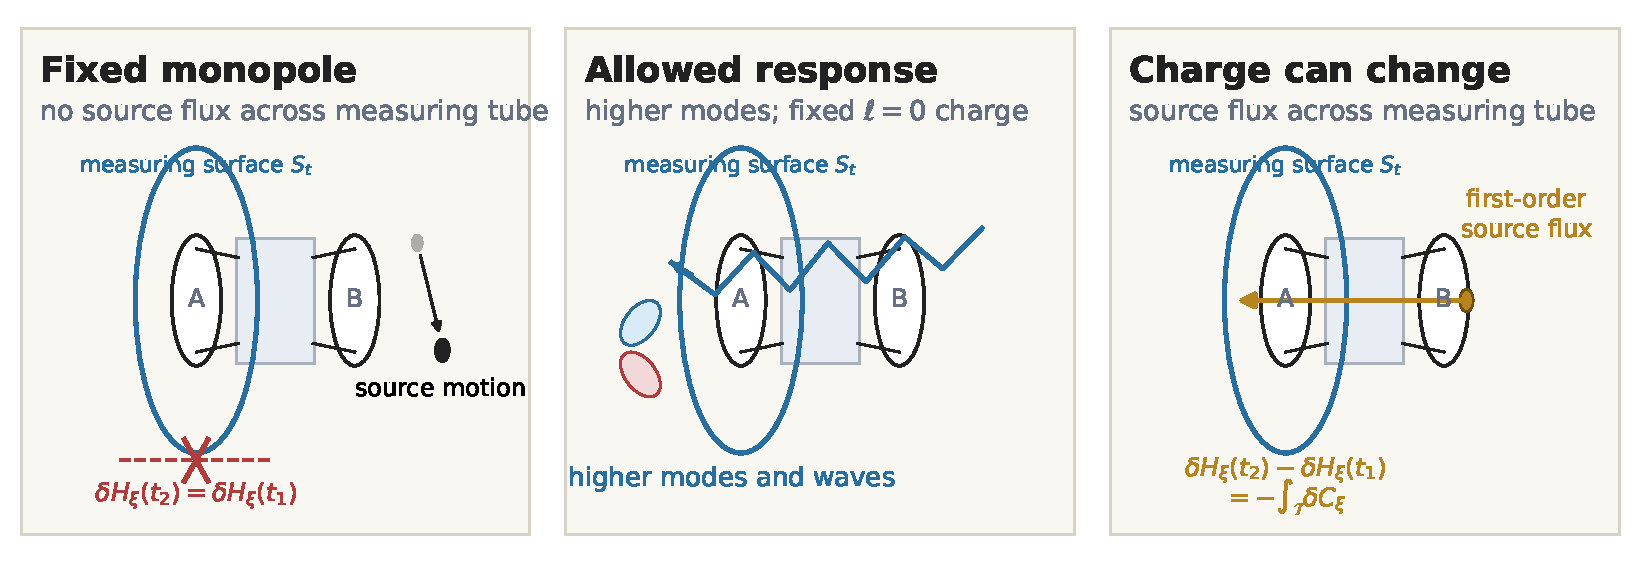
\includegraphics[width=0.98\textwidth]{fig_observer_charge_channels_v7.pdf}
  \caption{Balance-law channels.  With no first-order source flux through the
  observer-side measuring worldtube, the monopole charge is fixed (left).
  Higher multipoles and waves may still respond (center).  First-order matter
  or support-field flux can change the charge through
  Eq.~\eqref{eq:sourced-balance} (right).}
  \label{fig:channels}
\end{figure}

We use the standard Einstein--Hilbert representative of $\bm\theta$; with the
normalization of $\xi$ specified above, the charge agrees with the ADM mass
variation at an asymptotically flat end.
Gauge invariance here refers to proper diffeomorphisms that preserve the
measuring surface and the fixed asymptotic frame; a covariantly transformed
surface embedding is equivalent.  Large boundary time rescalings are not
gauge redundancies in this comparison.  The proof is local to $\mathcal T$, and
holds for a single-ended handle.

% ============================================================
\section{Application to the DS monopole}
\label{sec:gravity-application}
% ============================================================

On a round background sphere, harmonics with $\ell\ge1$ integrate to
zero, so $\delta H_\xi[S;h]$ sees only the $\ell=0$ part of the perturbation;
and because the linearized Einstein operator commutes with the harmonic
decomposition on a spherically symmetric background, that part satisfies the
monopole equations by itself.

With the background time normalization fixed, linearized Birkhoff
classification gives
\begin{equation}
  h^{\ell=0}_{\alpha\beta}
  =\delta M\,\partial_M\bar g_{\alpha\beta}
   +\mathcal L_\eta\bar g_{\alpha\beta},
  \label{eq:l0-mass}
\end{equation}
where $\eta$ generates an admissible gauge transformation
\cite{MartelPoisson2005SchwarzschildPerturbations}.  The vacuum field equations
make $\delta M$ constant in a connected first-order solution.  Since
$\partial_M\bar g$ is itself a vacuum perturbation, $d\bm k_\xi=0$ makes
$\int_S\bm k_\xi[\partial_M\bar g;\bar g]$ independent of the round sphere $S$
within the vacuum region.  With the standard Einstein--Hilbert representative
and the normalization of $\xi$ fixed above, a direct finite-sphere evaluation
gives this integral as unity.  Hence $\delta H_\xi[S;h]=\delta M$.  No sphere at
infinity is required for this equality; wherever an asymptotically flat end
exists, it agrees with the ADM mass variation.

For $r_g=2M$,
\begin{equation}
  \partial_M\bar g_{tt}=\frac{2}{r},
  \qquad
  \partial_M\bar g_{rr}=\frac{2r}{(r-r_g)^2}.
  \label{eq:mass-derivatives}
\end{equation}
Comparison with Eq.~\eqref{eq:ds-observer-mode} therefore identifies the
revised DS observer field as
\begin{equation}
  h^{\mathrm{our}}_{\alpha\beta}=b\,\partial_M\bar g_{\alpha\beta},
  \qquad
  \delta H_\xi=\delta M=b=\frac{\mu R}{A}.
  \label{eq:ds-is-charge}
\end{equation}

\begin{corollary}[DS mass-monopole rigidity]
Consider any on-shell completion of the DS construction about the stated
Schwarzschild background that retains
Eq.~\eqref{eq:ds-is-charge} and leaves a neighborhood of a fixed observer-side
measuring worldtube free of first-order constraint sources.  Then $b$ is
constant along the evolution.
\end{corollary}

\begin{proof}
Apply Theorem~\ref{thm:gravity} with the background Schwarzschild time
translation.  Equation~\eqref{eq:ds-is-charge} identifies its surface
functional with $b$.
\end{proof}

The prescription
\begin{equation}
  b(t)=\frac{\mu R}{A(t)}
  \label{eq:revised-time-dependent}
\end{equation}
instead moves through different mass-charge sectors as the source radius
changes.  Separate stationary solutions at different $A$ can exist without
being successive states of one source-free history.  The corresponding
bookkeeping is already standard: a mouth changes its mass when a body actually
transits it \cite{FrolovNovikov1990PhysicalEffects}.  Equation
\eqref{eq:revised-time-dependent} instead transfers mass between the two
mouths while nothing transits either one.%
\footnote{The revised static coefficients give
$\delta M_{\rm source}=\mu-\mu R/A$ and
$\delta M_{\rm observer}=\mu R/A$, whose sum is $\mu$ when each end uses its
future-directed unit time.  This is static bookkeeping, not a transfer law;
changing either charge requires the appropriate flux.}

There are two relevant ways an on-shell dynamical completion can alter this
conclusion.  If the $A(t)$-dependent part retains the mass-mode form, it changes
$\delta M$ and must be supplied by the source term in
Eq.~\eqref{eq:sourced-balance}.  If additional components instead make the
varying coordinate coefficient a gauge contribution, then it is not a mass
observable and the acceleration inferred from $h_{tt}$ alone requires a new
gauge-invariant derivation.  This exhausts the source-free first-order
$\ell=0$ sector in a fixed asymptotic frame; other physical channels remain.

In particular, nonspherical motion may generate $\ell\ge1$ perturbations and
radiative $\ell\ge2$ modes.  These do not contribute to the round-sphere mass
charge, but they may produce other observer-side effects.  In the DS
electrostatic model these carry their own geometric suppression: the matching
gives observer-side multipole coefficients proportional to
$R^{2\ell+1}/A^{\ell+1}$, so at observer radius $r_2$ the
dipole contribution to the potential is smaller than the monopole contribution
by $3R^2/(2Ar_2)$.  The gravitational analogues are not computed in the DS
construction, which treats the monopole alone
\cite{DaiStojkovic2019Observing}.  Vacuum
gravitational-wave energy flux is quadratic in first-order wave amplitude, so
over a fixed orbital time it is $O(\epsilon^2)$ rather than the reversible
$O(\epsilon)$ monopole modulation proposed in Eq.~\eqref{eq:ds-delta-a}
\cite{BondiVanderBurgMetzner1962Gravitational,Sachs1962Asymptotic}.  A
first-order matter or support-field flux is a distinct possibility already
covered by Eq.~\eqref{eq:sourced-balance}.  Nonlinear throat response and
scalar monopoles lie outside the present claim.

% ============================================================
\section{Conclusion}
\label{sec:conclusion}
% ============================================================

The DS calculation supplies a family of static fields labeled by the source
position.  For the spherical ansatz, a single component of the linearized
field equations already forbids the promotion $A\to A(t)$,
Eq.~\eqref{eq:momentum-constraint}.  Maxwell's equation settles the
electrostatic version exactly: each mouth carries a flux of its own, and
redistribution between them requires current across one of the surfaces.  The surface-charge identity gives the
general gravitational statement, valid for nonspherical perturbations and in
gauge-invariant form: the corrected DS observer coefficient is a first-order
Schwarzschild mass charge, and the worldtube balance holds it fixed in a
source-free evolution.

Fields still propagate through the wormhole, and the observer-side response is
nonzero.  Higher multipoles, waves, and explicit matter or support-field
dynamics remain available.  What does not
follow is the proposed position-dependent $O(\mu)$ mass monopole obtained by
the replacement $A\to A(t)$.  Establishing such a signal requires either the
first-order flux that changes the charge or a different gauge-invariant
observable.

\begin{acknowledgments}
The author thanks Ilia Slobodov for helpful discussions.
\end{acknowledgments}

\section*{AI Use Statement}

The author used OpenAI ChatGPT/Codex and Anthropic Claude as interactive
assistants for brainstorming, mathematical and editorial critique, prose
revision, consistency checks, reference searches, and figure preparation.  All
arguments, calculations, citations, figures, and conclusions were reviewed and
revised by the author, who is solely responsible for the manuscript.

\clearpage
\bibliographystyle{apsrev4-2}
\bibliography{references}

\end{document}
